\documentclass{standalone}
\usepackage{tkz-fct}
\usepackage{tkz-euclide}
\usepackage{color}
\usepackage{amsmath}
\renewcommand*\familydefault{\sfdefault}
\usepackage{sansmath}
\sansmath
\definecolor{gray75}{gray}{0.75}
\begin{document}
 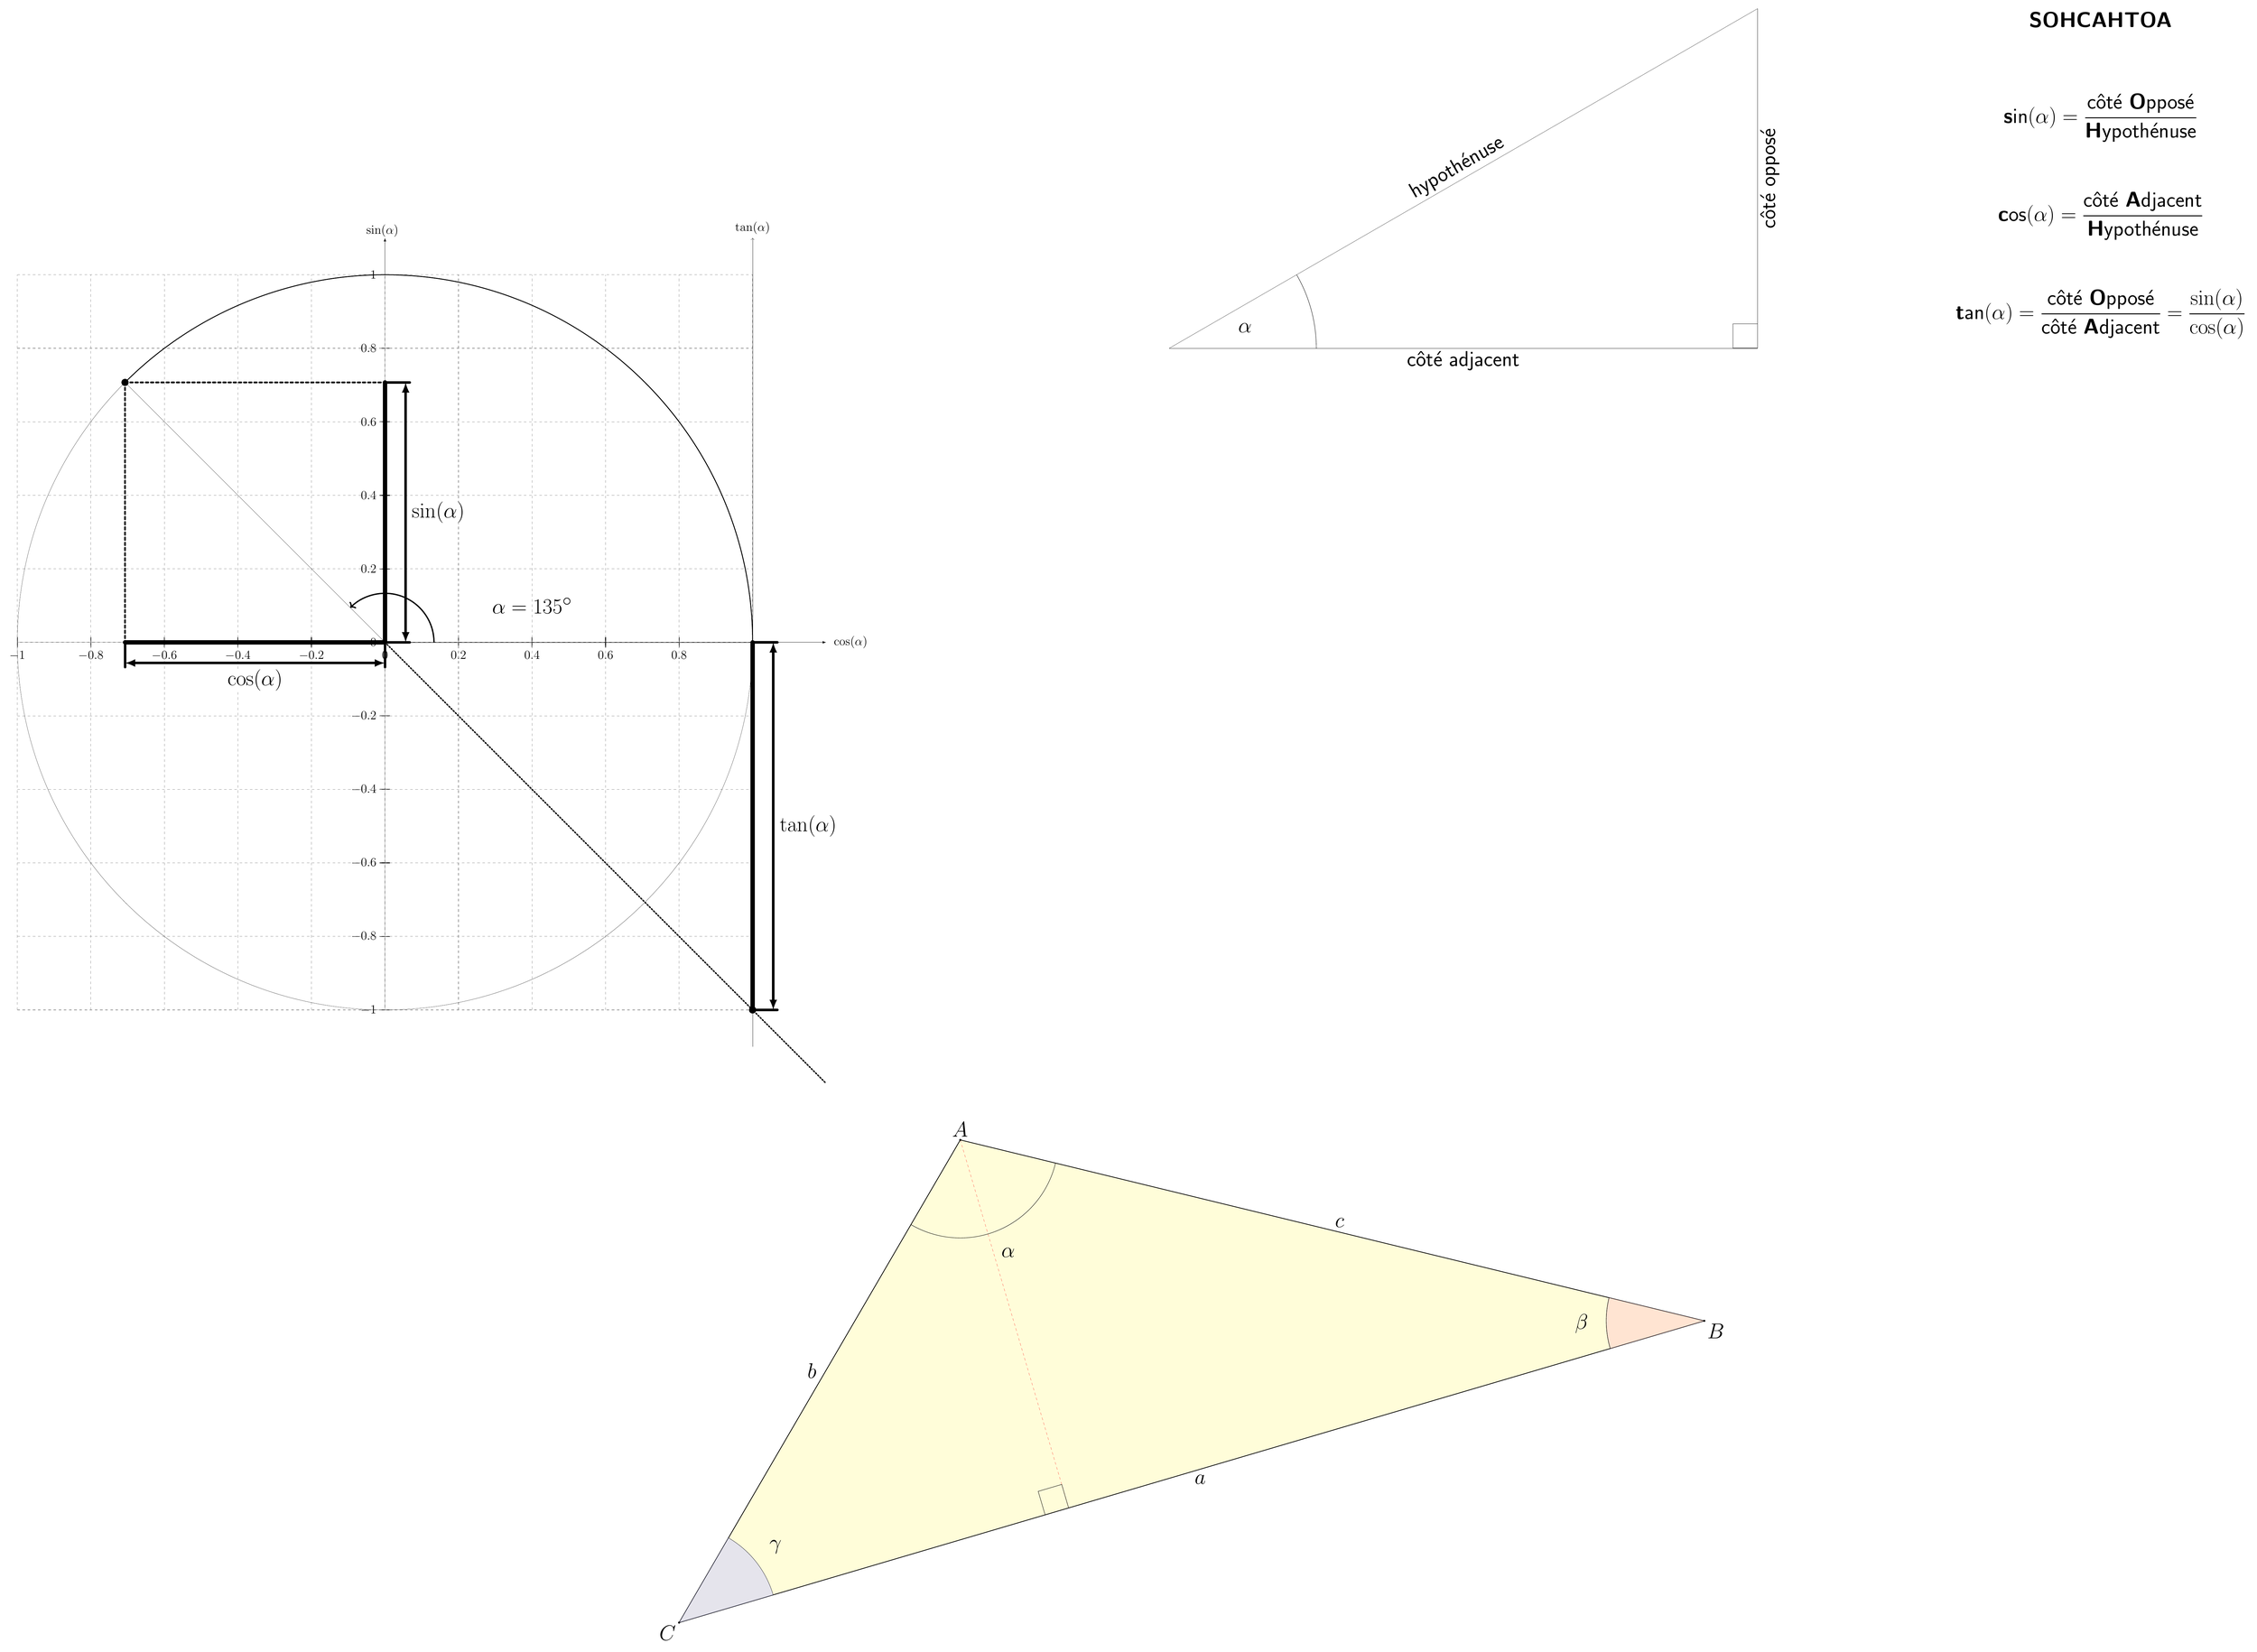
\begin{tikzpicture}[scale=2]
   \begin{scope}[scale=1.5]
    \tkzInit[xmax=1.,ymax=1.,xmin=-1. ,ymin=-1,xstep=0.2,ystep=0.2]
   \tkzDrawY[label=$\sin(\alpha)$, above, font=\Large]
   \tkzLabelY[node font=\Large]
   \tkzLabelX[node font=\Large]
   \tkzDrawX[label=$\cos(\alpha)$, right=8pt, font=\Large,right space=1]
   \tkzDefPoints{1/1.1/A,1/-1.1/B}
   \tkzDrawSegment[<-](A,B)
\tkzLabelSegment[line width=2pt, above, pos=0](A,B){\Large$\tan(\alpha)$}

   \begin{scope}[dashed]
     \tkzGrid
   \end{scope}
   \tkzDefPoints{0/0/O,1/0/A, 1/1/M,0/1/N}
   \tkzDrawCircle[color=black](O,A)
   \tkzDefPointBy[rotation= center O angle 135](A)
   \tkzGetPoint{P}
   \tkzDrawSegment(O,A)
   \tkzDrawSegment(O,P)
   \tkzDrawArc[color=black,line width=1pt](O,A)(P)
   \tkzDrawPoints(A,P,O)
   \tkzDrawPoint[size=8](P)
   \tkzPicAngle["",draw=black,
->,angle eccentricity=3,
angle radius=2cm, line width=1.5pt](A,O,P)
\tkzText(0.4,0.1){\Huge$\alpha=135^\circ$}
\tkzInterLL(O,P)(A,M)
\tkzGetPoint{Q}
\tkzDrawPoint[size=8](Q)
\tkzDrawLine[line width=1.5pt, add = 0 and .2, dotted](O,Q)
\tkzDefPointBy[projection= onto O--A](P)
\tkzGetPoint{PX}
\tkzDefPointBy[projection= onto O--N](P)
\tkzGetPoint{PY}
\tkzDrawSegments[dashed, line width=2pt](P,PX P,PY)
\tkzDrawSegments[line width=5pt](O,PX O,PY A,Q)
\tkzDrawSegment[line width=3pt,dim={\Huge$\cos(\alpha)$,24pt,below=6pt}](O,PX)
\tkzDrawSegment[line width=3pt,dim={\Huge$\sin(\alpha)$,-24pt,right=6pt}](O,PY)
\tkzDrawSegment[line
width=3pt,dim={\Huge$\tan(\alpha)$,24pt,right=6pt}](A,Q)
   \end{scope}
\begin{scope}[scale=2,xshift=8cm, yshift=3cm]
    \tkzDefPoints{0/0/A,6/0/B}
    \tkzDefTriangle[school](A,B)
    \tkzGetPoint{C}
    \tkzMarkRightAngles(C,B,A)
    \tkzLabelSegment[sloped](A,B){\Huge côté adjacent}
    \tkzLabelSegment[sloped](B,C){\Huge côté opposé}
    \tkzLabelSegment[above,sloped](A,C){\Huge hypothénuse}
    \tkzMarkAngle[size=1.5](B,A,C)
    \tkzLabelAngle[pos=0.8](B,A,C){\Huge $\alpha$}
    \tkzDrawSegments(A,B B,C C,A)
    \begin{scope}[yshift=-0.65cm,xshift=9.5cm]
    \tkzText(0,4){\bf\Huge SOHCAHTOA}
    \tkzText(0,3){\Huge $\text{{\bf s}in}(\alpha)=\dfrac{\text{côté {\bf
            O}pposé}}{\text{{\bf H}ypothénuse}}$}
    \tkzText(0,2){\Huge $\text{{\bf c}os}(\alpha)=\dfrac{\text{côté {\bf
            A}djacent}}{\text{{\bf H}ypothénuse}}$}
    \tkzText(0,1){\Huge$\text{{\bf t}an}(\alpha)=\dfrac{\text{côté {\bf
            O}pposé}}{\text{côté {\bf A}djacent}}=\dfrac{\sin(\alpha)}{\cos(\alpha)}$}
    \end{scope}
\end{scope}
\begin{scope}[scale=2,xshift=5cm,yshift=-10cm]
    \tkzDefPoint["\Huge $C$" below left](-2,0){C}
    \tkzDefPoint["\Huge $B$" below right](20:9){B}
    \tkzDefPoint["\Huge $A$" above](80:5){A}
    \tkzDefPointsBy[projection=onto B--C](A){a}
    \tkzDrawPolygon[thick,fill=yellow!15](A,B,C)
    \tkzDrawSegment[dashed, red](A,a)
    \tkzMarkAngle(B,C,A)
    \tkzMarkAngle(C,A,B)
    \tkzMarkAngle(A,B,C)
    \tkzMarkRightAngle(A,a,C)
    \tkzFillAngle[fill=blue!20, opacity=0.5](B,C,A)
    \tkzFillAngle[fill=red!20, opacity=0.5](A,B,C)
    \tkzLabelAngle[pos=1.25](A,B,C){\Huge $\beta$}
    \tkzLabelAngle[pos=1.25](B,C,A){\Huge $\gamma$}
    \tkzLabelAngle[pos=1.25](C,A,B){\Huge $\alpha$}
    \tkzLabelSegment[below right](C,B){\Huge $a$}
    \tkzLabelSegment[above left](A,C){\Huge $b$}
    \tkzLabelSegment[above right](A,B){\Huge$c$}
    \tkzMarkAngle(A,B,C)
    \tkzDrawPoints(A,B,C)
\end{scope}

\end{tikzpicture}
\end{document}
